\documentclass[11pt, letterpaper, titlepage]{article}
\usepackage[utf8]{inputenc}
\usepackage{hyperref}
\hypersetup{pdfborder=0 0 0}
\usepackage{amsmath}
\usepackage{amssymb}
\usepackage{geometry}
\usepackage[none]{hyphenat}
\usepackage{xcolor}
\usepackage{cite}
\usepackage{lipsum}
\usepackage{physics}
\usepackage{textgreek}
\usepackage{unicode-math}
\usepackage{subfigure}
\usepackage{graphicx}
\usepackage{textgreek}
\geometry{
 a4paper,
 left=25mm,%left=20mm,
 right=25mm,%right=20mm,
 bottom=25mm, %bottom=20mm,
 top=25mm,%top=20mm,
 }


%%%%%%%% PORTADA
\title{
 \textbf{\LARGE UNIVERSITY OF OSLO} \\
\vspace{37mm}
\textbf{\Large Project 1}\\
\vspace{7mm}
\Large FYS5419 – Project1
\vspace{25mm}
} 

\author{\Large Hishem Kløvnes }


        % \vspace{45mm}
        

\date{\Large 7 October 2024} % Deadline



\begin{document}
\maketitle
% \tableofcontents
\newpage




\section{a)}
In this project, there are a few matrices that will be used repetedly. So before doing anything, I will formulate them here first. 
The three Pauli matrices: 
\[
\begin{aligned}
σ_x &= \begin{pmatrix}  
        0 & 1 \\
        1 & 0
\end{pmatrix}\\
σ_y &= \begin{pmatrix}
        0 &-i\\
        i & 0
\end{pmatrix}\\
σ_z  &= \begin{pmatrix}
      1 & 0\\
      0 &-1  
\end{pmatrix}
\end{aligned}
\] 
The Hadamard and Phase gate
\[
\begin{aligned}
        H &= \frac{1}{\sqrt{2}} \begin{pmatrix}
                1&1\\1&-1
        \end{pmatrix}\\
        S &= \begin{pmatrix}
                1&0\\0&i
        \end{pmatrix},
\end{aligned}
\]
and the CNOT gate
\[
\begin{aligned}
        CNOT &= \begin{pmatrix}
                1&0&0&0\\
                0&1&0&0\\
                0&0&0&1\\
                0&0&1&0
        \end{pmatrix}
\end{aligned}
\]

In this part of the project, the goal was to take a one qubit basis, apply the right gates to it - creating a Bell state - and then measure the state. The states we use are simply \(\ket{0} = [1,0]\) and \(\ket{1} = [0,1]\). The Bell state is given by
\[
\begin{aligned}
        \ket{\Phi^+} &= \frac{1}{\sqrt{2}}(\ket{00} + \ket{11})\\
        \ket{\Phi^-} &= \frac{1}{\sqrt{2}}(\ket{00} - \ket{11})\\
        \ket{\Psi^+} &= \frac{1}{\sqrt{2}}(\ket{01} + \ket{10})\\
        \ket{\Psi^-} &= \frac{1}{\sqrt{2}}(\ket{01} - \ket{10})
\end{aligned}
\]
where $\ket{00}$ is the state where both qubits are in the state $\ket{0}$, and $\ket{11}$ is the state where both qubits are in the state $\ket{1}$. \newline
The first thing I did was to apply the Hadamard gate and the Phase gate to the one qubit basis to see what happens. 
\[
\begin{aligned}
H \ket{0} &= \frac{1}{\sqrt{2}}\begin{pmatrix}
        1&1\\1&-1
\end{pmatrix}
\begin{pmatrix}
  1\\0
\end{pmatrix} = \frac{1}{\sqrt{2}} \begin{pmatrix}
        1\\1
\end{pmatrix}\\
H \ket{1} &= \frac{1}{\sqrt{2}}\begin{pmatrix}
        1&1\\1&-1
\end{pmatrix}
\begin{pmatrix}
        0\\1
\end{pmatrix} = \frac{1}{\sqrt{2}}\begin{pmatrix}
        1\\-1
\end{pmatrix}\\
\end{aligned}
\] 
This means that after applying the Hadamard gate to the one-qubit basis, we get a pair of new states which are defined as superpositions of the original states. Here the new superpositioned states are almost identical. The only difference is the sign of the second state, which represents that the state points along \(-X\) axis on the bloch sphere, in contrast to the first state which points along the \(X\) axis. \newline
The next step was to apply the Phase gate to the one-qubit basis.
\[
\begin{aligned}
S \ket{0} &= \begin{pmatrix}
        1&0\\0&i
\end{pmatrix}
\begin{pmatrix}
        1\\0
\end{pmatrix} = \begin{pmatrix}
        1\\0
\end{pmatrix}\\
S \ket{1} &= \begin{pmatrix}
        1&0\\0&i
\end{pmatrix}
\begin{pmatrix}
        0\\1
\end{pmatrix} = \begin{pmatrix}
        0\\i
\end{pmatrix}
\end{aligned}
\]
This means that the Phase gate does not change the state of the qubit in the $\ket{0}$ state, but it changes the state of the qubit in the $\ket{1}$ state. The \(\ket{1}\) state still points to the south pole of the block sphere, but has acquired a phase factor of \(i\). \newline
The next step was to define Bell states. To do this, I first defined them explicitly, and then I created the Bell states by applying the right gates to each state. As I mentioned earlier there are four Bell states, and to create them I applied the CNOT and Hadamard gates to different tensor products of the one-qubit basis.
\[
\begin{aligned}
CNOT &⋅ (H \ket{0}) ⊗ \ket{0} = \frac{1}{\sqrt{2}} [1,0,0,1]\\
CNOT &⋅ (H \ket{1}) ⊗ \ket{0} = \frac{1}{\sqrt{2}} [0,1,1,0] \\
CNOT &⋅ (H \ket{0}) ⊗ \ket{1} = \frac{1}{\sqrt{2}} [1,0,0,-1] \\
CNOT &⋅ (H \ket{1}) ⊗ \ket{1} = \frac{1}{\sqrt{2}} [0,1,-1,0]
\end{aligned}
\]
I double checked these states with the definition of the Bell states, and they are correct. The next step was to apply the Hadamard gate and thereafter the CNOT gate to the Bell states. Let's take the first Bell state as an example. 
\[
\begin{aligned}
CNOT &⋅ (H ⊗ I) \ket{\Phi^+} = \\
CNOT &⋅ \frac{1}{\sqrt{2}} \begin{pmatrix}
        1&1\\1-1
\end{pmatrix} ⊗ \begin{pmatrix}
        1&0\\0&1
\end{pmatrix} \ket{\Phi^+} =\\
CNOT &⋅ \frac{1}{\sqrt{2}} \begin{pmatrix}
        1&0&1&0\\0&1&0&1\\1&0&-1&0\\0&1&0&-1
\end{pmatrix} \ket{\Phi^+} =\\
CNOT &⋅ \frac{1}{2} \begin{pmatrix}
        1\\0\\0\\-1 
\end{pmatrix} = \frac{1}{2} \begin{pmatrix}
        1&0&0&0\\0&1&0&0\\0&0&0&1\\0&0&1&0
\end{pmatrix} \begin{pmatrix}
        1\\1\\1\\-1
\end{pmatrix} = \frac{1}{2} \begin{pmatrix}
        1\\1\\-1\\1
\end{pmatrix}
\end{aligned}
\]
When repeating this process for all our Bell states, we notice that all of them are superpositions of all states: \(\ket{00}, \ket{01}, \ket{10}, \ket{11}\). This means that it does not matter which of the modified Bell states we use to measure, because the outcome should be the same. \newline
\begin{figure}
        \begin{center}
                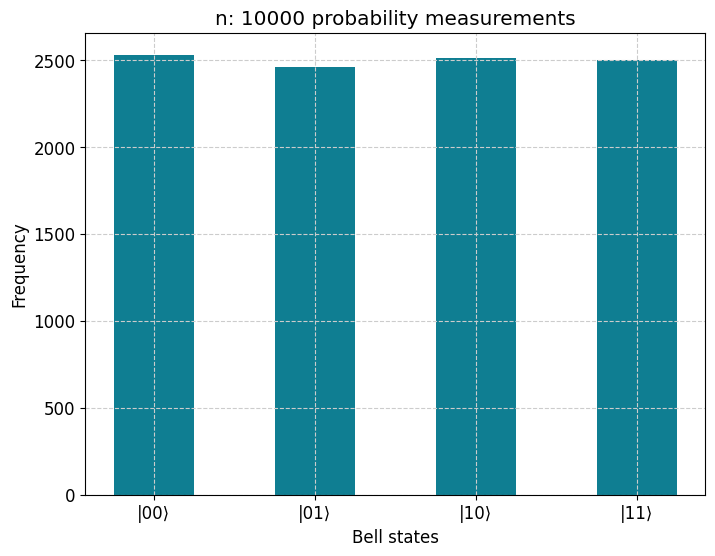
\includegraphics[scale=0.3]{BellMeasurement.png}
                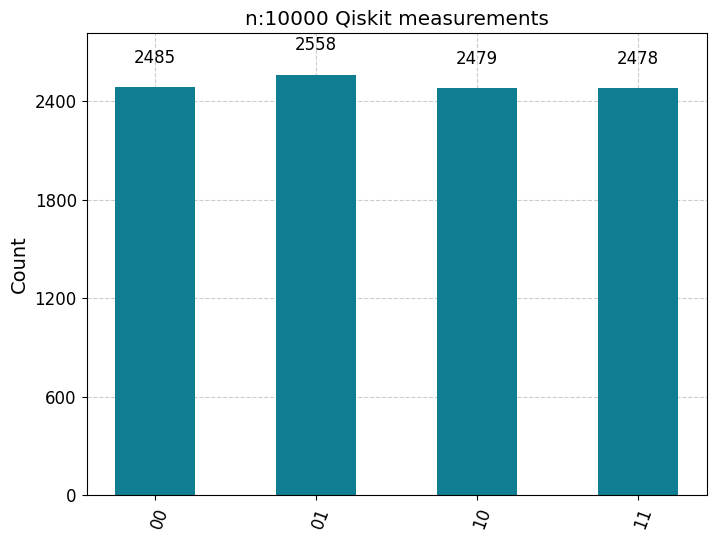
\includegraphics[scale=0.3]{BellMeasurementQiskit.png}       
        \end{center}
        \caption{The left figure shows the measurement of the Bell states using the method described above. The right figure shows the measurement of the Bell states using Qiskit.}
        \label{fig:BellMeasurement}
\end{figure}
In \ref{fig:BellMeasurement} Ihave compared the measurement of the Bell states using the method described above with the measurement of the Bell states using Qiskit. I did \(n=10000\) measurement on both methods, and the results are practically identical, which is what we would expect. For a system like this, we would expect the results to be around 25\% for each state. If we were to do even more measurements, \(n = 100000,1000000\cdots   \) we would expect the results to be even closer to 25\% for each state. \newline


\section{b)}
For this part of the problem, we have the same one-qubit basis as in the previous problem. Now we have a Hamiltonian \(H = H_0 + λH_I\), where
\[
H_0 = \mathcal{E} I + Ω σ_z, \quad \mathcal{E} = \frac{E_{1} + E_2}{2}, \quad Ω = \frac{E_1 - E_2}{2}
\]
and 
\[
H_I = cI + ω_zσ_z + ω_xσ_x
\]
where \(
c = (V_{11}+V_{22})/2, \quad ω_z = (V_{11}-V_{22})/2, \quad ω_x = V_{12}=V_{21}
\). We have a set of given values for our parameters:
\(E_1=0, E_2=4, V_{11}=V_{-22}=3, V_{12} = V_{21}=0.2\). \newline
In this section we want to find the eigenvalues of the Hamiltonian when acted on the one-qubit basis, as a function of the parameter \(λ\). This was solved numerically. 
\begin{figure}
  \begin{center}
        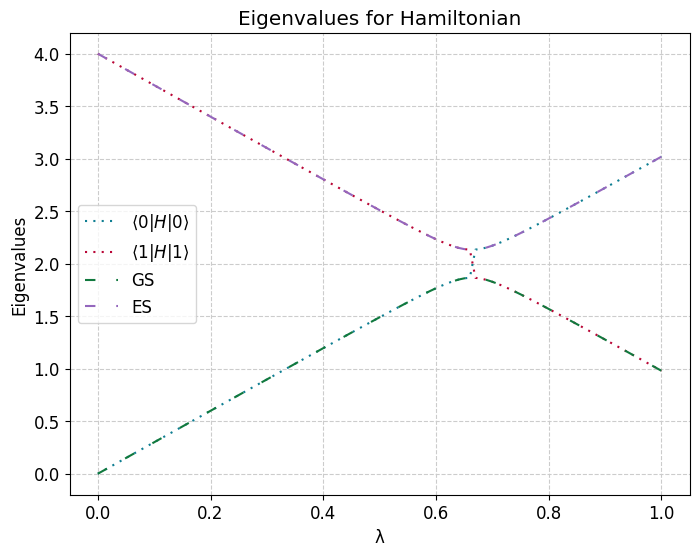
\includegraphics[scale=0.7]{Eigvals.png}
        \caption{The eigenvalues of the Hamiltonian as a function of the parameter \(λ\). ES represents the excited state, and GS represents the ground state.}
  \end{center}
\end{figure}







\end{document}











